\chapter{Introducción}

El crecimiento exponencial en el uso de tecnologías móviles y plataformas de comunicación digital ha transformado la manera en que interactúan las personas. Según datos de la ENDUTIH 2023 \cite{UsoInternetPorEstado}, en México el 81.2\,\% de la población utiliza teléfono celular y el 96.1\,\% de los usuarios de internet en la Ciudad de México lo hace para comunicarse, principalmente a través de redes sociales y aplicaciones de mensajería. Esta adopción masiva ha traído consigo grandes beneficios, pero también ha abierto nuevas oportunidades para la comisión de delitos como el \textit{catfishing} y la extorsión digital.

La facilidad con la que se pueden crear perfiles falsos y establecer contacto anónimo en entornos digitales ha hecho que estos delitos proliferen, afectando especialmente a los jóvenes, quienes presentan la mayor penetración de internet (96.7\,\% en el grupo de 18 a 24 años). Además, cifras del INEGI (ENVIPE 2023) \cite{ENVIPE2023} reflejan un repunte en la tasa de incidencia de fraudes y extorsiones, situando a este fenómeno como una amenaza persistente en el ámbito digital.

El presente trabajo concentrara sus esfuerzos sobre las estafas catfishing y sextorsión puntualmente.

\textbf{A lo largo del presente trabajo se encuentra una variedad de terminología de diferentes áreas del saber, se recomienda  consultar la sección glosario en la cual se definen todas aquellas palabras que a lo largo del trabajo estan escritas en itálica denotando ser un término presente en la sección antes mencionada.
}

\subsubsection{Personas usuarias de tecnologías de la información y comunicación}

\begin{figure}[H]
    \centering
    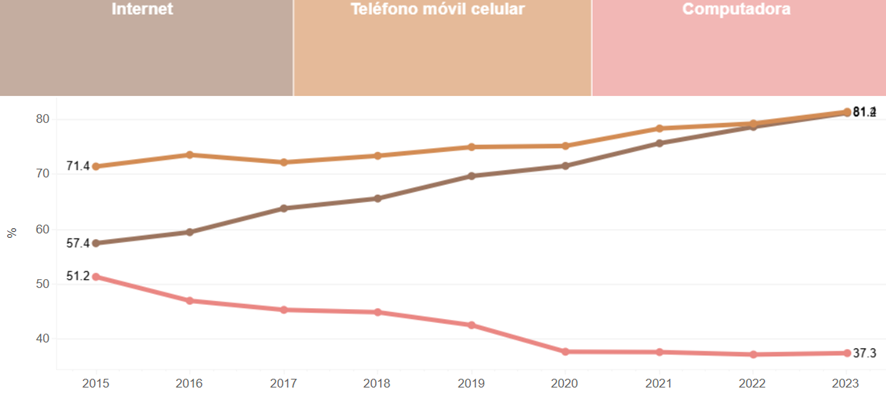
\includegraphics[width=1\linewidth]{imagenes/grafica1.png}
    \caption{orcentaje de usuarios de internet, telefonía móvil y computadora en México, 2023. Adaptado de Encuesta Nacional sobre Disponibilidad y Uso de Tecnologías de la Información en los Hogares (ENDUTIH)2023, por Instituto Nacional de Estadística y Geografía, 2024,\url{https://www.inegi.org.mx/programas/endutih/2023/\#informacion_general}.
    {\textcopyright} INEGI}
    \label{fig:1}
\end{figure}

\begin{figure}[H]
    \centering
    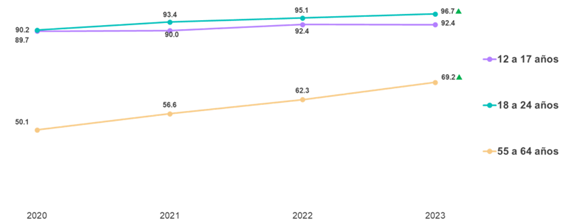
\includegraphics[width=1\linewidth]{imagenes/grafica2.png}
    \caption{Personas usuarias de internet según grupos de edad del 2020 al 2023\newline
    Acceso a internet por entidad federativa, 2023. Tomado de Encuesta Nacional sobre Disponibilidad y Uso de Tecnologías de la Información en los Hogares (ENDUTIH) 2023: Comunicado de prensa núm. 161/24, por Instituto Nacional de Estadística y Geografía, 2024, \url{https://www.inegi.org.mx/contenidos/saladeprensa/boletines/2024/ENDUTIH/ENDUTIH_23.pdf}. {\textcopyright} INEGI}
    \label{fig:2}
\end{figure}

Datos de la ENDUTIH 2024 muestran que los jóvenes de 18 a 24 años presentan la mayor penetración
de Internet en México (96.7 \%), lo cual coincide con su alta participación en redes sociales y aplicaciones de
citas. Esta combinación los convierte en un grupo con mayor exposición a estafas románticas y catfishing

\begin{figure}[H]
    \centering
    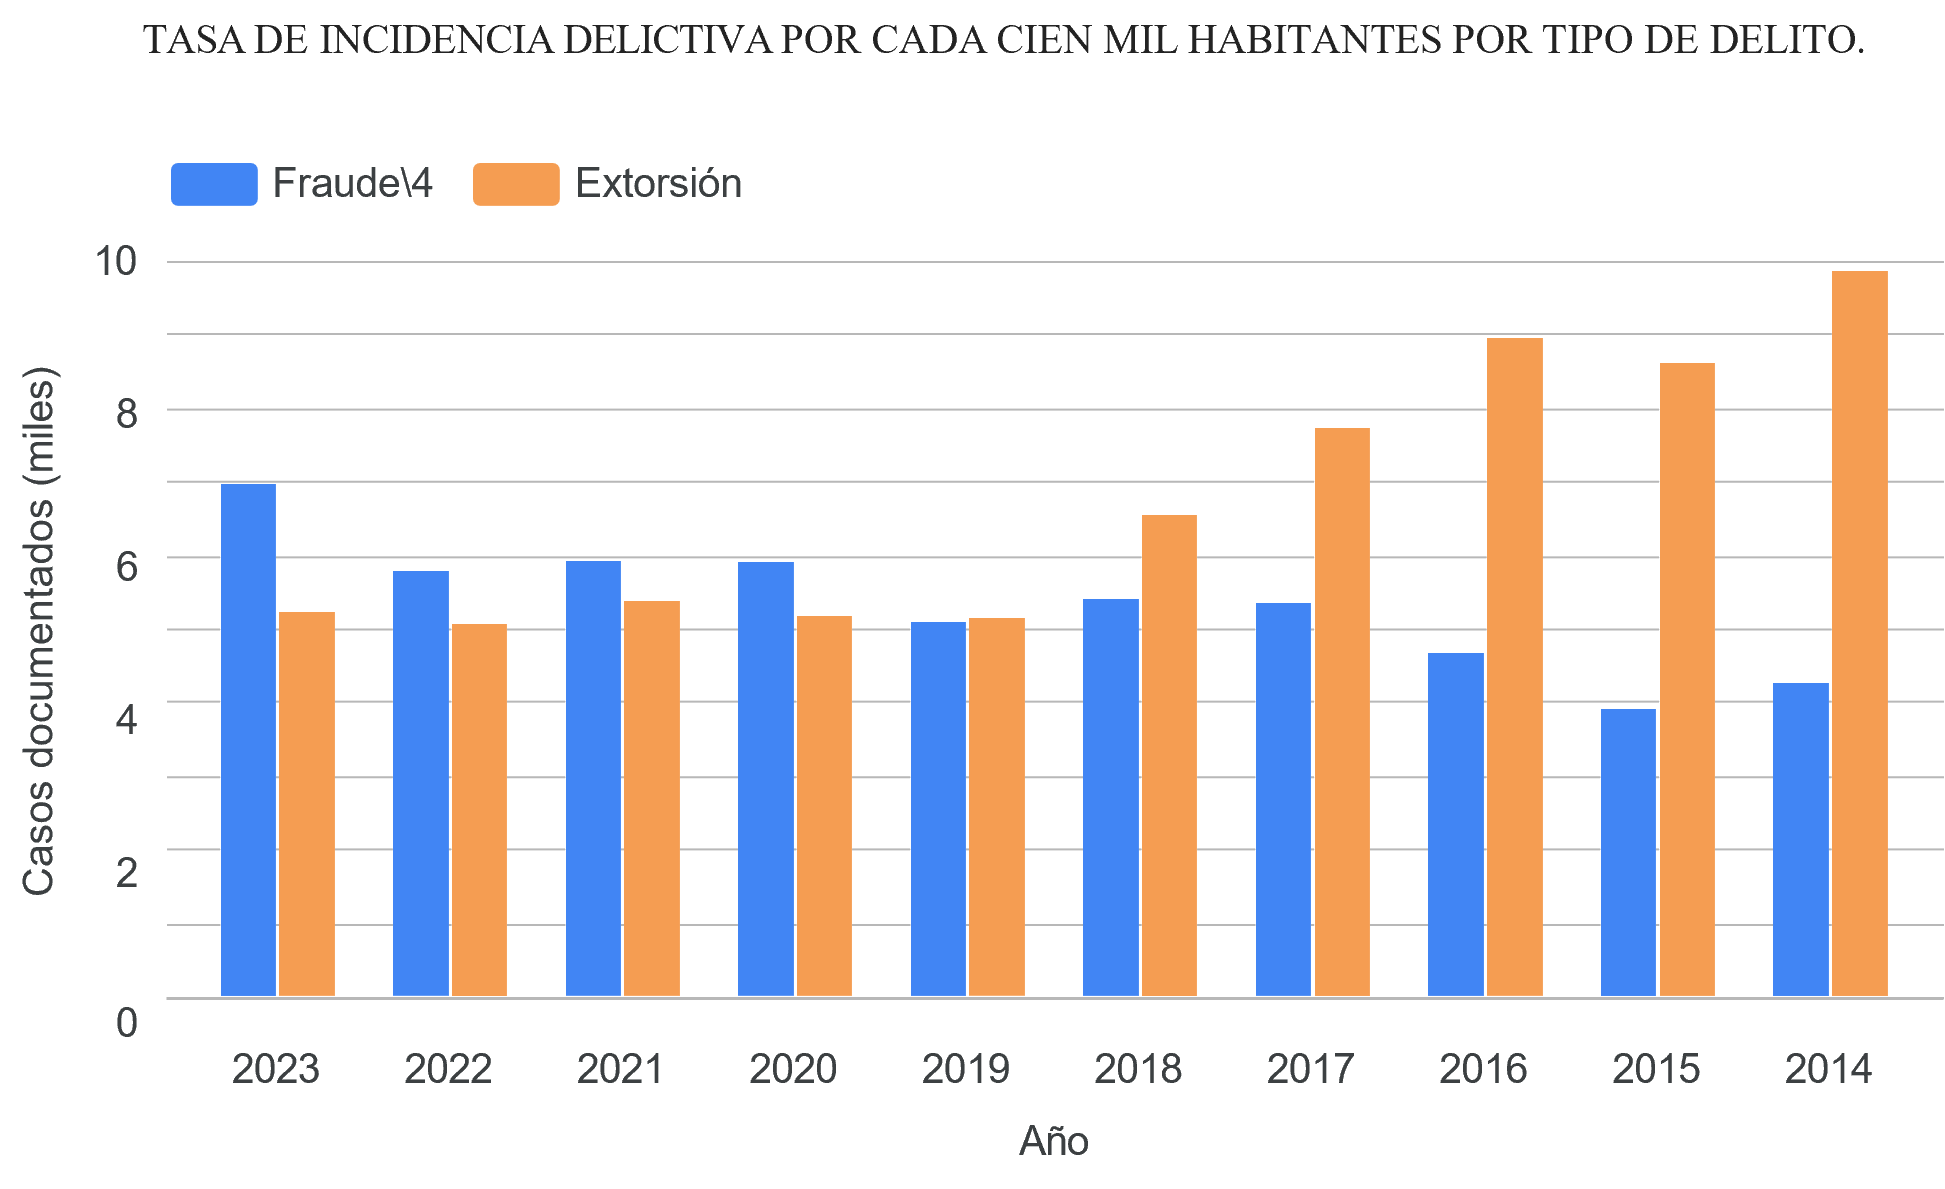
\includegraphics[width=1\linewidth]{imagenes/Tasa de incidencia delictiva por cada cien mil habitantes por tipo de delito..png}
    \caption{\cite{ENVIPE2023}}
    \label{fig:enter-label}
\end{figure}

\subsubsection{Servicios con los que cuenta la población}

Según la encuesta “Hogares con equipamiento de tecnología de información y comunicaciones, por entidad
federativa, según tipo de tecnología, 2023” en los hogares de la ciudad de México se cuentan con los servicios
de Internet 89.5 \%, telefonía 98.9 \%

\cite{ENDUTIH2023}

\subsubsection{Propósitos del uso de internet}

Según la base de datos “Usuarios de internet, por entidad federativa, según principales usos, 2023”, El
96,1 \% de los 7,897,062 de personas encuestadas en la ciudad de México , utilizan el ¿ para comunicarse, el
90,7 \% para redes sociales, el 37.7 \% para realizar operaciones bancarias, el 1.3 para pagos con tarjetas de
prepago.\cite{ENDUTIH2023}